%% AASTeX requires revtex4-1.cls (http://publish.aps.org/revtex4/) and
%% other external packages (latexsym, graphicx, amssymb, longtable, and epsf).
%% All of these external packages should already be present in the modern TeX 
%% distributions.  If not they can also be obtained at www.ctan.org.

%% The first piece of markup in an AASTeX v6.x document is the \documentclass
%% command. LaTeX will ignore any data that comes before this command. The 
%% documentclass can take an optional argument to modify the output style.
%% The command below calls the preprint style which will produce a tightly 
%% typeset, one-column, single-spaced document.  It is the default and thus
%% does not need to be explicitly stated.
%%
%%
%% using aastex version 6.3
\documentclass[twocolumn]{aastex63}

%% The default is a single spaced, 10 point font, single spaced article.
%% There are 5 other style options available via an optional argument. They
%% can be invoked like this:
%%
%% \documentclass[arguments]{aastex63}
%% 
%% where the layout options are:
%%
%%  twocolumn   : two text columns, 10 point font, single spaced article.
%%                This is the most compact and represent the final published
%%                derived PDF copy of the accepted manuscript from the publisher
%%  manuscript  : one text column, 12 point font, double spaced article.
%%  preprint    : one text column, 12 point font, single spaced article.  
%%  preprint2   : two text columns, 12 point font, single spaced article.
%%  modern      : a stylish, single text column, 12 point font, article with
%% There are other optional arguments one can invoke to allow other stylistic
%% actions. The available options are:
%%
%%   astrosymb    : Loads Astrosymb font and define \astrocommands. 
%%   tighten      : Makes baselineskip slightly smaller, only works with 
%%                  the twocolumn substyle.
%%   times        : uses times font instead of the default
%%   linenumbers  : turn on lineno package.
%%   trackchanges : required to see the revision mark up and print its output
%%   longauthor   : Do not use the more compressed footnote style (default) for 
%%                  the author/collaboration/affiliations. Instead print all
%%                  affiliation information after each name. Creates a much 
%%                  longer author list but may be desirable for short 
%%                  author papers.
%% twocolappendix : make 2 column appendix.
%%   anonymous    : Do not show the authors, affiliations and acknowledgments 
%%                  for dual anonymous review.
%%
%% these can be used in any combination, e.g.
%%
%% \documentclass[twocolumn,linenumbers,trackchanges]{aastex63}
%%
%% AASTeX v6.* now includes \hyperref support. While we have built in specific
%% defaults into the classfile you can manually override them with the
%% \hypersetup command. For example,
%%
%% \hypersetup{linkcolor=red,citecolor=green,filecolor=cyan,urlcolor=magenta}
%%
%% will change the color of the internal links to red, the links to the
%% bibliography to green, the file links to cyan, and the external links to
%% magenta. Additional information on \hyperref options can be found here:
%% https://www.tug.org/applications/hyperref/manual.html#x1-40003
%%
%% Note that in v6.3 "bookmarks" has been changed to "true" in hyperref
%% to improve the accessibility of the compiled pdf file.
%%
%% If you want to create your own macros, you can do so
%% using \newcommand. Your macros should appear before
%% the \begin{document} command.
%%

\usepackage{float}
\usepackage{amsmath}
\usepackage{amsfonts}

\newcommand{\vdag}{(v)^\dagger}
\newcommand\aastex{AAS\TeX}
\newcommand\latex{La\TeX}

%% Reintroduced the \received and \accepted commands from AASTeX v5.2
%\received{June 1, 2019}
\revised{\today}
%\accepted{\today}
%% Command to document which AAS Journal the manuscript was submitted to.
%% Adds "Submitted to " the argument.
%\submitjournal{AJ}


%% You can add a light gray and diagonal water-mark to the first page 
%% with this command:
%% \watermark{text}
%% where "text", e.g. DRAFT, is the text to appear.  If the text is 
%% long you can control the water-mark size with:
%% \setwatermarkfontsize{dimension}
%% where dimension is any recognized LaTeX dimension, e.g. pt, in, etc.
%%
%%%%%%%%%%%%%%%%%%%%%%%%%%%%%%%%%%%%%%%%%%%%%%%%%%%%%%%%%%%%%%%%%%%%%%%%%%%%%%%%
\graphicspath{{./}{figures/}}
%% This is the end of the preamble.  Indicate the beginning of the
%% manuscript itself with \begin{document}.

\newcommand{\f}[2]{\frac{#1}{#2}}
\begin{document}

\title{A Review of Astrophysical Black Holes}

\correspondingauthor{Aayush Arya}
\email{aayush.11912610@lpu.in}

\author{Aayush Arya}
\affiliation{Lovely Professional University \\
Jalandhar-Delhi-G.T. Road\\
Phagwara, Punjab 144411, India}

%\nocollaboration{1}

%% Mark off the abstract in the ``abstract'' environment. 
\begin{abstract}

Black holes are compact objects with density so high that the escape velocity at their surfaces exceeds the speed of light. Such objects were initially thought to have no physical existence. The discovery of a black hole component in the X-ray binary system Cygnus-X1 convinced astrophysicists about their existence. They are found in galaxies scattered as stellar mass black holes, as well at the center of most massive galaxies as supermassive black holes (SMBHs). Black holes are believed to play an important role in galaxy evolution. We discuss the importance of black holes in astrophysical phenomena and highlight key recent discoveries, including the direct observations announced by the EHT Collaboration, detection of gravitional radiation emitted by binary black hole merging events by the LIGO and Virgo Collaborations.

\end{abstract}

%% the Keywords should appear after the \end{abstract} command. 
%% See the online documentation for the full list of available subject
%% keywords and the rules for their use.
\keywords{black holes, stellar mass --- gravitational waves --- AGN --- galaxy evolution}

%% We recommend that authors also use the natbib \citep
%% and \citet commands to identify citations.  The citations are
%% tied to the reference list via symbolic KEYs. The KEY corresponds
%% to the KEY in the \bibitem in the reference list below. 

\section{Introduction} \label{sec:intro}

\subsection{Black Hole Studies: The Past and the Present}

For any given object of mass $M$, the escape velocity of a particle having mass $m$ bound by its gravitational potential well can be obtained by equating the sum of kinetic energy and potential energy of the particle to zero
$$ \f{1}{2}mv^2 - \f{GMm}{r} = 0$$
Physically, this means that the particle $m$ shall lose all its kinetic energy when it escapes the potential well to infinity. The idea applies to all objects regardless of mass. From this, the idea of "dark stars" from which even light couldn't escape was first speculated indepedently by Michell (1783) and Laplace (1796). From Newtonian dynamics, one can calculate that the escape velocity of an object exceeds the speed of light if it's radius is smaller than

$$
    r_s = \frac{2GM}{c^2} 
$$

where $r_s$ is called the \textit{Schwarzschild radius}. The \textit{Schwarzschild solution}, presented by Karl Schwarzschild in 1916 just a year after Einstein formulated his field equations, was the first description of a spherically symmetric, non-rotating, electrically uncharged black hole. Further developments by the 1960s gave the \textit{Kerr-Newman solution} which describes the spacetime around a spherically symmetric, rotating and charged black hole.\\

It became known that black holes are relatively simple in the sense that they can be completely described using just three parameters \textemdash their mass $M$, spin angular momentum $J$, and electric charge $Q$. This is based on certain assumptions and is known as the \textit{no-hair theorem}.

The formation of black holes is believed to be a result of stellar collapse of massive stars. When the nuclear fuel is depleted in massive stars, the electron and neutron degeneracy pressures after a certain limit can no longer prevent the gravitational collapse and when the radius of the collapsing object becomes smaller than its Schwarzschild radius, it becomes a black hole. Cygnus-X1 is the brightest X-ray binary source in the sky, discovered in 1964. The mass of one of its components, estimated by studying the orbital motion of its companion, was found to be greater than the maximum mass for a neutron star. Cygnus-X1 thus became the first confirmed candidate for a stellar-mass black hole and convinced the astrophysics community about the physical existence of black holes.\\

Recent investigations of gravitational radiations by the LIGO and Virgo collaborations have reported events that are reminiscient of binary black hole mergers. In April 2018, using the Event Horizon Telscope, the EHT collaboration announced the breakthrough discovery of the first picture of a black hole. In this paper, we will review these recent studies and also discuss the importance of black holes in astrophysical systems, such as in nuclei of active galaxies and evolution of galaxies themselves. We acknowledge that several excellent reviews on black holes already exist (\cite{bambi2019astrophysical}; \cite{Capelo_2019}) and that some of content is inherited from them.

\section{Observational Signatures}
\subsection{Accretion from Companion: Stellar-mass Black Holes}
Stellar-mass black holes lie in the mass range of $3-100$ M$_{\odot}$ (\cite{Capelo_2019}) and are believed to form upon the death of massive stars. When a star depletes its fusion capacity and is no longer able to counter its own gravitational pull by virtue of the electron and neutron degeneracy pressures, the stellar core starts to collapse. This is believed to produce stellar-mass black holes.\\

Initial evidence for the existence of stellar-mass black holes came from the study of a subclass of binary stars called X-ray binaries (\cite{Casares_2006}). As most stars exist in pairs, if one of the stars explodes and forms a compact object such as a neutron star or a black hole, it will start accreting material from its companion. When material from a companion stars falls on the surface of a black hole, it is accelerated to relativistic speeds and due to internal friction, the debris glows in X-rays.\\ Cygnus-X1, discovered in 1961, was a binary source identified to host a O9.47lab supergiant. The existence of an unseen companion was determined by radial velocity measurements. 
It had a peak radial velocity of ~64 km s$^{-1}$ (which was later refined to be around 75 km s$^{-1}$ and a period of ~5.6 days.\\

\begin{figure}
    %\centering
    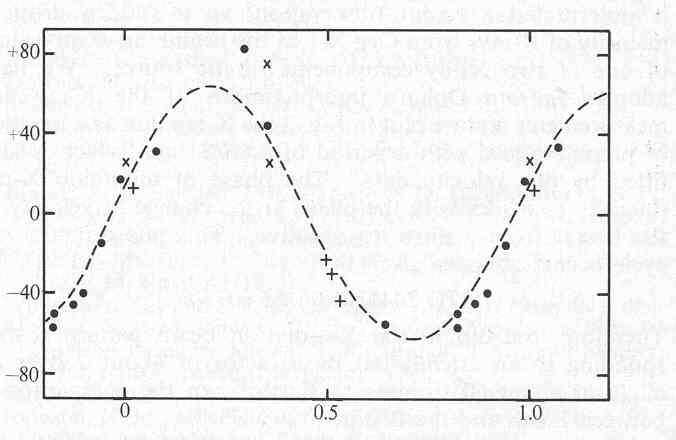
\includegraphics[width=0.5\textwidth]{cygx1_curves.png}
    \caption{Radial velocity (km s$^{-1}$) curve of the companion star in Cygnus-X1. Reprinted from \cite{1972Natur.235...37W}}
    \label{fig:cygx1_radial}
\end{figure}

After accounting for uncertainties in distance, for inclination angle $i$, calculations using the time period of orbit $P_{orb}$, and mass of the visible companion $M_c$, the mass of the unseen compact object $M_x$ was constrained to be $\geq 4$M$_{\odot}$ (\cite{BoltonCYGX1}).   It had been shown that under certain assumtions, the maximum mass of a neutron star can be constrained to be $3.2\pm 0.2$ M$_{\odot}$ (\cite{Rhoades&Ruffini}). Therefore, Cygnus-X1 was a strong black hole candidate. Such a discovery was important in the field to establish the physical existence of these extraordinary objects.

\subsection{Supermassive Black Holes}
Supermassive Black Holes (SMBHs) lie in the mass range of $10^5$ to $10^{10}$ M$_\odot$ and are believed to exist at the centers of most large galaxies. Our own Milky Way galaxy has a central supermassive black hole found to coincide with the position of Sagittarius A* (\cite{Ghez1998ApJ...509..678G}).\\

These black holes have unusual physical propeties that make their behavior distinct from stellar mass black holes. Since the density of a black hole is inversely proportional to the square of the mass, higher mass black holes have lower average density (\cite{2015eiub.book.....B}) than stellar-mass black holes.

The formation of these unusual objects remains to be an open problem. However, it is believed that black holes can grow by accretion of matter and galaxy merger events (\cite{2015ApJ...799..178K}). These black holes are thought to be the driving engines of some of the most energetic astrophysical processes, such as luminous emissions from quasars. They reside in the cores of active galaxies, known as \textit{active galactic nuclei}. There is also a correlation between the mass of a central black hole and the mass of its host galaxy, as discussed in Section \ref{subsec:coevolution}. Due to this, some experts believe that there is a black holes and galaxies \textit{coevolve}. We describe the direct evidence of supermassive blackholes at the center of the M87 galaxy in Section \ref{EHTsection}.\\

\subsubsection{Active Galactic Nuclei}

Active Galactic Nuclei (AGNs) are the compact cores of galaxies that exhibit very high luminosity emissions and are found to emit in the entirety of the electromagnetic spectrum, from radio to $\gamma-$rays. They are the most powerful sources of non-explosive emission in the universe and are visible up to very high redshifts. One of the most distant quasars, at redshift $z = 7.085$ was reported by \cite{2011Natur.474..616M}. These emissions have been theorized to be due to accretion of matter by the central SMBHs and can't be explained as stellar-emissions. Galaxies that host an AGN are known as \textit{active galaxies}. The most powerful AGNs, called \textit{quasars}, could have luminosities thousands of times greater than that of a galaxy like Milky Way (\cite{2015Natur.518..512W}). The Sloan Digital Sky Survey reported more than 500,000 quasars (\cite{P_ris_2018})\\

Current models suggest that when cold material gets within the sphere of influence of the central SMBH, it becomes a source of accretion. Just like accretion discs in the case of X-ray binaries,  the material gets heated due to frictional forces and emits electromagnetic radiation. The expected peak in the emission spectrum of an AGN is in the optical-UV range.

\begin{figure}[H]
    \centering
    \includegraphics[width=0.40\textwidth]{m87-jet.jpg}
    \caption{The relativistic jet of the active galaxy M87, extending for more than 5,000 light years. The blue jet resulting from synchrotron radiation contrasts from the emission from the galaxy's starlight (yellow). Image Credit: NASA/Hubble Heritage Team (STScI/AURA)}
    \label{fig:m87_jet}
\end{figure}

In addition to that, a hot corona may form above the accretion disk which may inverse-Compton scatter photons upto X-ray energies.

Some AGNs produce twin, collimated, relativistic jets that emerge from close to the disc that may extend upto thousands of light years. These jets emit radiation via routes of synchrotron radiation as well as inverse-Compton scattering.The properties, such as the observed luminosity of quasars depend on various factors such as rate of accretion of material, size of the central black hole, orientation of the galaxy.

\subsubsection{Direct Searches: the Event Horizon Telescope} \label{EHTsection}
In April 2019, the first direct image of the supermassive blackhole at the centre of the M87 active galaxy was reported by \cite{2019ApJ...875L...1E}. This was a breakthrough discovery as no previous telescope was capable of resolving the objects of such compact size. The high resolution was obtained using Very Large Baseline Interferometry (VLBI) techinques. 

\begin{figure}[H]
    \centering
    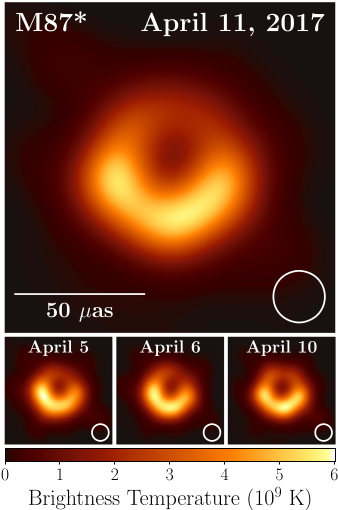
\includegraphics[width=0.4\textwidth]{eht_m87_cb.png}
    \caption{Top: EHT Image of M87*. The image is an average of three images produced by different imaging methods. North is top, East is left. Bottom: similar images taken on different days, showing the stability of the basic image structure. Colour bar shows temperature scale. Figure reprinted from \cite{2019ApJ...875L...1E}}
    \label{fig:eht_image}
\end{figure}

In VLBI, data are recorded at different telscope stations, with the use of extremely precise atomic clocks locked onto GPS time standards for synchronzing the time of arrival of the signal at different antenna. This allows recording the source coherently. VLBI essentially gives a baseline equivalent to the maximum separation between the telescopes. and the EHT Collaboration, making use of telescopes across the world, was able to get a baseline comparable to the size of the Earth.\\

In the EHT collaboration image (Figure \ref{fig:eht_image}), the central dark region is the region inside the event horizon of the black hole from w hich light cannot escape. The glowing circular ring is the heated plasma of the accretion disk, which can be seen because it occupies the photon sphere outside the event horizon. The conspicuous North-South asymmetry in the ring is due to the spin of the black hole.

The shadow of the black hole observed is consistent with predictions of the general theory of relativity, making the theory pass an extremely important test.

\section{Importance}

\subsection{Black Hole-Galaxy Co-evolution} \label{subsec:coevolution}
One of the great revolutions made by the Hubble Space Telescope was that it allowed quantitative study of black hole demographics. An important discovery made by such investigations was that in any galaxy, the mass of the central black hole was tightly correlated with the bulge of the rest of the galaxy (\cite{2003ApJ...589L..21M}), leading to the belief that black holes and galaxies \textit{co-evolve} by regulating each other's growth. A recent review highlighted that sometimes black holes of mass $10^5-10^6$M$_{\odot}$ are found in many bulgeless galaxies and do not necessarily correlate with galaxy disks (\cite{2013ARA&A..51..511K}).\\

It is argued that that jets, radiation and winds from the Active Galactic Nucleus can interact with the interstellar medium surrounding it and can heat up or even eject the gas, preventing star formation. This itself may devoid the feeder black hole of its fuel and halt its growth. Numerical simulations show that this feedback is necessary to explain the properties of massive galaxies. \cite{Mart_n_Navarro_2018} showed that black-hole mass scales with the gas cooling rate in the early Universe. Quenching of star formation was reported to happen earlier in galaxies with larger mass central black holes. Therefore, central SMBHs are believed to regulate star formation in galaxies.

\subsection{Gravitational Radiation from Merger Events}
In 1916, Albert Einstein predicted the existence of gravitational waves a year after he formulated his field equations. The linearized weak-field equations had a wave solutions \textemdash they were transverse waves travelling at the speed of light. However, until the Chapel Hill conference in 1957, there was no significant debate on the existence of gravitational waves. In 2016, the LIGO and Virgo Collaborations reported the direct detection of gravitational waves by a binary black hole merging event (\cite{PhysRevLett.116.061102}).\\

The LIGO detectors are modified Michelson interferometers in which laser light from a 20W laser source is split into two arms of length 4km each using a beam splitter. The two halves of the beam recombined after travelling different paths.  Passage of gravitational waves would stretch each of the arms differently, since they are oritented perpendicular to each other. Changes to the length of the paths or the time taken for the two split beams, to reach the point where they recombine are revealed as beats. This can provide extremely sensitive detections, of changes in length of spacetime of size smaller than the diameter of a proton ($10^{-15}$ m).

Such detection events from merger events, apart from being tests of Einsteinian gravity, may provide new insights into the nature of gravity itself.

\section{Conclusions}
Black holes are an important prediction of Einstein's general theory of relativity. They are known to play a central role in many astrophysical phenomena, including the activity of galactic nuclei and evolution of galaxies themselves.Initially, their including physical existence was inferred from the study of X-ray binaries. In 2019, by recording a direct image, the EHT Collaboration has provided the strongest evidence for the existence of black holes till date. Gravitational radiation from binary black hole merger events studied by GW detectors such as LIGO and Virgo may provide new insights into our understanding of gravity itself.
%% For this sample we use BibTeX plus aasjournals.bst to generate the
%% the bibliography. The sample63.bib file was populated from ADS. To
%% get the citations to show in the compiled file do the following:
%%
%% pdflatex sample63.tex
%% bibtext sample63
%% pdflatex sample63.tex
%% pdflatex sample63.tex

\bibliography{paper_bib}{}
\bibliographystyle{aasjournal}

%% This command is needed to show the entire author+affiliation list when
%% the collaboration and author truncation commands are used.  It has to
%% go at the end of the manuscript.
%\allauthors

%% Include this line if you are using the \added, \replaced, \deleted
%% commands to see a summary list of all changes at the end of the article.
%\listofchanges

\end{document}

% End of file `sample63.tex'.
